\chapter{Ensayos y resultados}

\label{cap:EnsayosResultados}

En este capítulo se describe la fase de investigación previa al desarrollo del dispositivo de captura, junto con las pruebas realizadas para validar su correcto funcionamiento, tanto en un entorno de laboratorio como en una formación de Trenes Argentinos.

\section{Capturas del tráfico de la red en una formación}
\label{sec:capturas}

Como parte de la etapa de investigación, se realizó en junio de 2020 una visita al taller Victoria de Trenes Argentinos, coordinada por Sergio Dieleke (Coordinador Laboratorio Electrónico, Subgerencia de Material Rodante Línea Mitre). El objetivo principal de la visita fue tomar capturas del tráfico del bus MVB, para tomar conocimiento acerca del estándar TCN y de la implementación particular en las EMU de Trenes Argentinos.

Para tomar las capturas se conectó un MAX485 y un analizador lógico VKTECH entre dos dispositivos MVB.
También se utilizó un osciloscopio para verificar que la señal capturada tuviera las características esperadas.
En la figura~\ref{fig:banco-capturas} se muestra un diagrama de bloques del banco de medición.
En las figuras~\ref{fig:foto-banco-capturas} y \ref{fig:osciloscopio} se muestra una fotografía del banco de medición y un detalle de la señal capturada en el osciloscopio.

% video con la secuencia https://drive.google.com/drive/folders/1I-V33ElLX13Iy0YliUeojRwYFQKuucAO
\begin{figure}[htbp]
	\centering
    {
        \fontfamily{phv}
        \fontsize{9pt}{9pt}\selectfont
        \input{./Figures/banco-captura.pdf_tex}
    }
	\caption{Banco de medición utilizado para tomar las capturas.}
    \label{fig:banco-capturas}
\end{figure}

\begin{figure}[htbp]
	\centering
	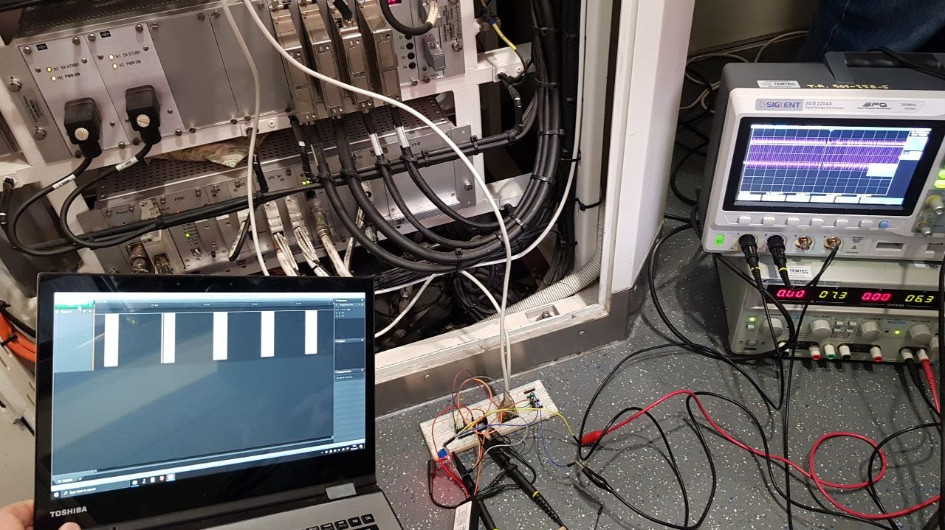
\includegraphics[width=\textwidth]{./Figures/foto-capturas.jpg}
	\caption{Fotografía del banco de medición utilizado para tomar las capturas.}
    \label{fig:foto-banco-capturas}
\end{figure}

\begin{figure}[htbp]
	\centering
	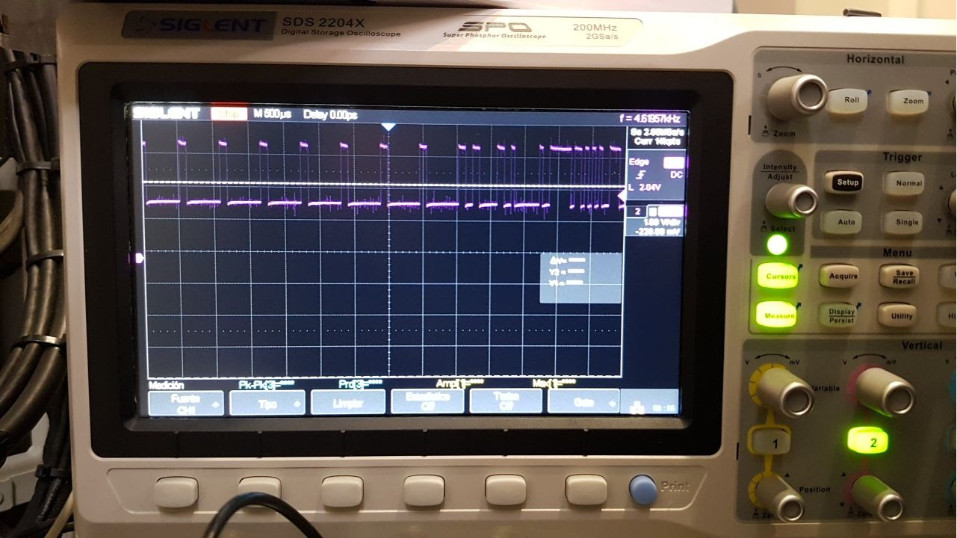
\includegraphics[width=\textwidth]{./Figures/osciloscopio.jpg}
	\caption{Señal MVB capturada en el osciloscopio.}
    \label{fig:osciloscopio}
\end{figure}

Mediante la PC conectada con el analizador lógico se tomaron capturas de un minuto de duración del tráfico del bus MVB, con el banco de medición conectado en diferentes puntos del segmento.
En simultáneo con las capturas se efectuó el procedimiento de encendido de la red y una secuencia de pasos tales como tomar cabina, abrir y cerrar puertas, cambio de marcha, etc., de forma tal de generar tráfico en la red y así poder analizar en detalle el funcionamiento de la misma.

En la figura~\ref{fig:pulseview} se muestra una visualización de una de las capturas.
En la figura~\ref{fig:pulseview-10ms} se observa que en los primeros 10ms se transmitieron 10 telegramas, aunque en el nivel de detalle no es suficiente para discernir su formato.
En la figura~\ref{fig:pulseview-telegrama} se amplía la visualización de uno de los telegramas, donde se puede apreciar en detalle las tramas \textit{master} y \textit{slave}.
Estas visualizaciones se obtuvieron utilizando el software PulseView, que es parte del proyecto Sigrok.

\begin{figure}[htbp!]
	\centering
    \begin{subfigure}[b]{\textwidth}
        \centering
        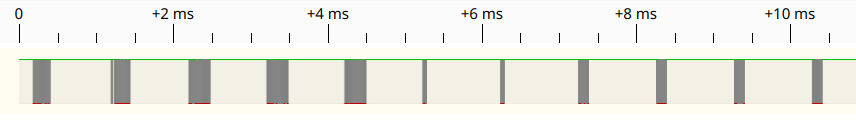
\includegraphics[width=\textwidth]{./Figures/pulseview-10ms.png}
        \caption{Algunos telegramas transmitidos en el transcurso de 10 ms.}
        \label{fig:pulseview-10ms}
    \end{subfigure}
    \par\bigskip
    \begin{subfigure}[b]{\textwidth}
        \centering
        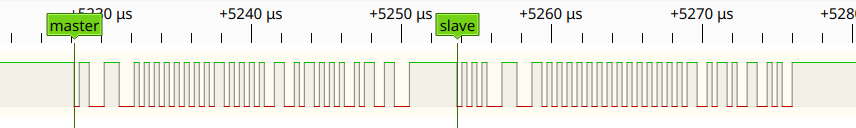
\includegraphics[width=1\textwidth]{./Figures/pulseview-telegrama.png}
        \caption{Ampliación de un telegrama.}
        \label{fig:pulseview-telegrama}
    \end{subfigure}
    \caption{Visualización de una de las capturas realizadas.}
    \label{fig:pulseview}
\end{figure}

\section{Decodificación de las capturas}
\label{sec:decodificacion}

\section{Pruebas con el generador de señal}
\section{Captura en tiempo real}
